% \newcommand{\prototitle}{Versuch 2 - Statistik}
% \newcommand{\Fachbereich}{Praktikum Messtechnik}
% \input{../packages/tu_header}

\newcommand{\institut}{Institut f\"ur Telekommunikationssysteme}
\newcommand{\fachgebiet}{Nachrichten\"ubertragung}
\newcommand{\veranstaltung}{Praktikum Nachrichten\"ubertragung}
\newcommand{\pdfautor}{\"Ozg\"u Dogan (326 048), Boris Henckell (325 779)}
\newcommand{\autor}{\"Ozg\"u Dogan (326 048)\\ Boris Henckell (325 779)}
\newcommand{\gruppe}{Gruppe: D03}
%\newcommand{\betreuer}{Betreuer: Mahmoud Felk}


\newcommand{\pdftitle}{Nachrichten\"ubertragung\ Praktikum\ 04}
\newcommand{\prototitle}{Praktikum 04 \\ Pulsamplitudemodulation und nichtideale Abtastung}


\input{../../packages/tu_header_8}
%\begin{document}

% \lstlistoflistings
\definecolor{darkgray}{rgb}{0.95,0.95,0.95}
\definecolor{darkolivegreen}{HTML}{01a801}
\definecolor{functionsBlue}{HTML}{32b9b9}
\definecolor{variableRed}{rgb}{1,0,0}
\definecolor{stringBrown}{HTML}{bc8e8e} % f geht nicht

\lstset{
        %\lstset{extendedchars=true} % Umlaute an der richtigen stelle und nicht am Anfang ausgeben
        %basicstyle=\footnotesize\ttfamily,
        basicstyle=\small,
        %
        inputencoding=utf8,
        %
        tabsize=4,
        showspaces=false,
        showtabs=false,
        showstringspaces=true, % no special string spaces
        %
        backgroundcolor=\color{darkgray}, % background
        stringstyle=\color{stringBrown}\fseries, % Strings
        keywordstyle=\color{functionsBlue}\bfseries, % keywords Blau
        identifierstyle=\color{variableRed}, % variablen
        commentstyle=\color{darkolivegreen}, %  comments
        %
        breaklines=true,
        %
        numbers=left,
        numberstyle=\tiny,
        stepnumber=1,
        numbersep=7pt,
        %
        frame=single,
        columns=flexible,
        %
        xleftmargin=-2cm,
        xrightmargin=-1.5cm,
        %
        language=Matlab
}

%---------------------------------------------------------------------
%---------------------------------------------------------------------
%---------------------------------------------------------------------


\section{Einleitung}
\begin{quote}
	\TODO{Einleitung so okay?}
	In diesem Termin werden zwei nichtideale Abtastverfahren für die
	Rekonstruktion eines PAM-modulierten Signals untersucht. Diese zwei Verfahren
	sind das Abtastung durch Signalausblendung (shape-top sampling) und die
	Abtastung mit Signalverbreiterung (flat-top sampling). Beide Verfahren werden
	im Zeit- und im Frequenzbereich untersucht, dabei werden ihre Auswirkungen auf
	die Rekonstruktion der abgetasteten Signale interpretiert.
\end{quote}%beende Einleitung
%--------------------------------------------------------------------
%--------------------------------------------------------------------    


\section{Theorie}
\begin{quote}
	\subsection{Abtastung durch Signalausblendung (shape-top sampling)}
    \begin{quote}  
        \TODO{Theorie einfügen}
        
    \end{quote}
    
    \subsection{Abtastung mit Signalverbreiterung (flat-top sampling)}
    \begin{quote}
    	\TODO{Theorie einfügen}
    \end{quote}

    
    \subsection{Vorbereitungsaufgabe}
    \begin{quote}        
        Zunächst werden die Formeln für das Spektrum eines abgetasteten Signals
        hergeleitet. Das $\alpha$ steht dabei für das Tastverhältnis.
        
        \subsubsection{Shape-Top-Sampling}
        \begin{quote}
            \begin{equation*}
                \begin{split}
                    f_m (t)   &= f(t) \cdot \sqcap_{\alpha T} (t) \ast \delta_T (t) \\
                    F_S (j\omega) &= \frac{1}{2\pi} F (j\omega) \ast \left [
                    \alpha T \cdot si \left( \frac{\omega \alpha T}{2} \right) \cdot \omega_T \cdot \delta_{\omega T} (\omega) \right] \\
                    &= \alpha \cdot F (j \omega) \ast \left ( si \left( \frac{\omega \alpha T}{2} \right)
                    \sum_{k=-\infty}^{\infty} \delta (\omega - k\omega_T) \right)\\
                    &= \alpha \cdot F (j \omega) \ast \sum_{k=-\infty}^{\infty} (si(k \pi \alpha) \cdot \delta (\omega -
                    k\omega_T))\\
                    &= \alpha \cdot \sum_{k=-\infty}^{\infty} \left [ si(k \pi \alpha) \cdot F (j(\omega - k\omega_T))
                    \right]\\
                \end{split}
            \end{equation*}
        \end{quote}
        
        \subsubsection{Flat-Top-Sampling}
		\begin{quote}
			\begin{equation*}
            	\begin{split}
            		f_m (t) &= [f (t) \cdot \delta_T (t)] \ast \sqcap_{\alpha T} (t)\\
            		F_F (j\omega) &= \left ( \frac{1}{2 \pi} F (j\omega) \ast \omega_T
            		\cdot \delta_T (\omega) \right) \cdot \alpha T \cdot si (\frac{\alpha \omega T}{2})\\
            		&= \alpha \cdot si \left( \frac{\omega \alpha T}{2} \right) \cdot \sum_{k=-\infty}^{\infty} F(j(\omega -
            		k\omega_T))\\
            	\end{split}
            \end{equation*}
		\end{quote}
		
		Danach werden die resultierenden Spektren $F_S (j\omega)$ und $F_F (j\omega)$
		für das Nutzsignal
		\begin{equation*}
        f(t) = A \cdot cos(\frac{\omega_T}{5}t)    	
        \end{equation*}
		mit $\alpha = 0.5$ und $\omega_T = 20\pi kHz$.
		
		
		 \begin{figure}[H]
    \centering
        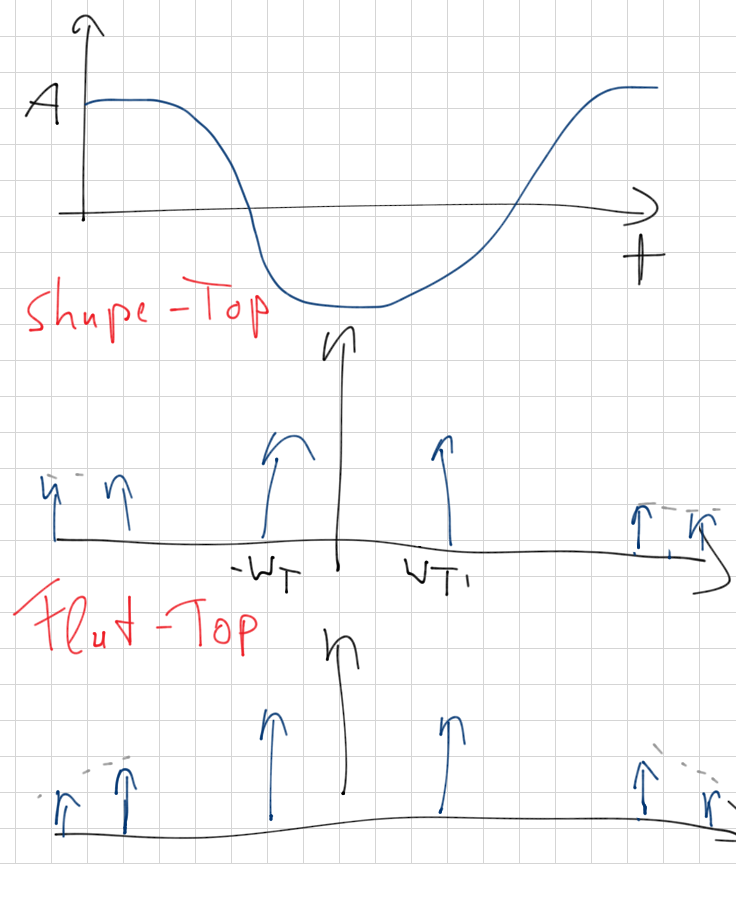
\includegraphics[scale=0.7, trim = 0cm 0cm 0cm 0cm,
        clip]{./Bilder/Vorbereitungskizze}
            \caption{Skizze}
  	    \end{figure}
    
    	Es ist zu sehen, dass sich die Spektren in Abhängigkeit von $\alpha$
    	verändern.
    	\TODO{wie genau muss noch eingefügt werden + ein vllt schöneres Bild -
    	falls überhaupt schöner möglich ist}
    	
    	Außerdem wird die Planung zur Praktikumsdurchführung im voraus gemacht. Für
    	den Versuch haben wir uns folgendes überlegt\ldots
    	\TODO{Stichwortartige Beschreibung über die Realisierung des Aufbau,
    	Blockschaltbilder einfügen, erwähnen wo wichtige Messungen gemacht werden
    	sollen}
    	
    	Zuletzt wird eine MATLAB-Simulation der Abtastung mittels Signalausblendung
    	und Signalverbreiterung für ein Sinussignal als Quellsignal und der
    	Abtastfrequenz von $400 kHz$.
    \TODO{Vorbereitungsaufgaben beenden}
    \end{quote}%subsection beenden

\end{quote}%Theorie beeanden
    
    \section{Labordurchführung}
    \begin{quote}
         \TODO{Durchführung schreiben}
   	\end{quote}%beende Labordurchführung
    	    
    
    \section{praktische Umsetzung}
    \begin{quote}
    Die praktische Umsetzung des Versuchs ist für beide Abtastverfahren gleich.
    
    \TODO{zu Ende bringen}
    \end{quote}%beende praktische Umsetzung
    
    
    \section{Auswertung}
    \begin{quote}    
        \TODO{Auswertung schreiben}
    \end{quote}%beende Auswertung
    
    \section{Zusammenfassung}
    \begin{quote}
    	\TODO{Zusammenfassung schreiben}
    \end{quote}%beende Zusammenfassung

%--------------------------------------------------------------------
%--------------------------------------------------------------------            

\TODO{Boris: öfter mal ein Überraschungsgeschenk für deine beste Freundin
besorgen!!}

%--------------------------------------------------------------------
%--------------------------------------------------------------------    


\begin{thebibliography}{999}
% \bibitem {AMohnetraeger} Prof. Dr.-Ing. Sikora, Thomas; Prof. Dr.-Ing. Noll, Peter: Einführung in die
% Nachrichtenübertragung, S.207




%Name, Vorname.; evtl. Name2, Vorname2.: Titel des Dokumentes
%oder Buches, Zeitschrift/Verlag/URL (Auflage, Erscheinungsort, -jahr), ggf. Seitenzahlen
% \bibitem {PasevalscheTheorem} \url{https://de.wikipedia.org/wiki/Parsevalsches_Theorem}, Zugriff
% 23.05.2012
\end{thebibliography}

\end{document}
